\documentclass{beamer}

\usepackage{fontspec}
\usepackage{float}

%\setmainfont{STSong}
\setmainfont{STHeitiSC-Light}
%\setmainfont{Hei}

%\setsansfont{STSong}            % Set Title font
\setsansfont{Hei}            % Set Title font

\setmonofont{STSong}

\usetheme{metropolis}           % Use metropolis theme

\usepackage{graphicx}

\title{人工智能的哲学思考}
\date{2018 3/12} 
\author{葛天逸,陈东箭,李陈豪,王韧,张思钧}
\institute{马克思主义基本原理概论课堂讨论} 
\begin{document}
  \maketitle
  \tableofcontents

  \section{人工智能的定义}
  \begin{frame}{人工智能的定义}
  \end{frame}



  \section{人工智能的人权问题}
  \begin{frame}{人工智能的人权问题}
    \begin{itemize}
     \item 人权:人因其为人而应享有的权利
     \item 人工智能脱胎于人类文化
     \item 「人权」的概念服务于人类自身  
     \item 如果人工智能可融入人类,那么「意识」为何
    \end{itemize}
  \end{frame}

  \section{人工智能未来发展}

  \begin{frame}{人工智能未来发展}
    \begin{itemize}
     \item  如果未来机器拥有了人性,人类该如何自处?
    \end{itemize}
   \begin{figure}[H]
   \centering
   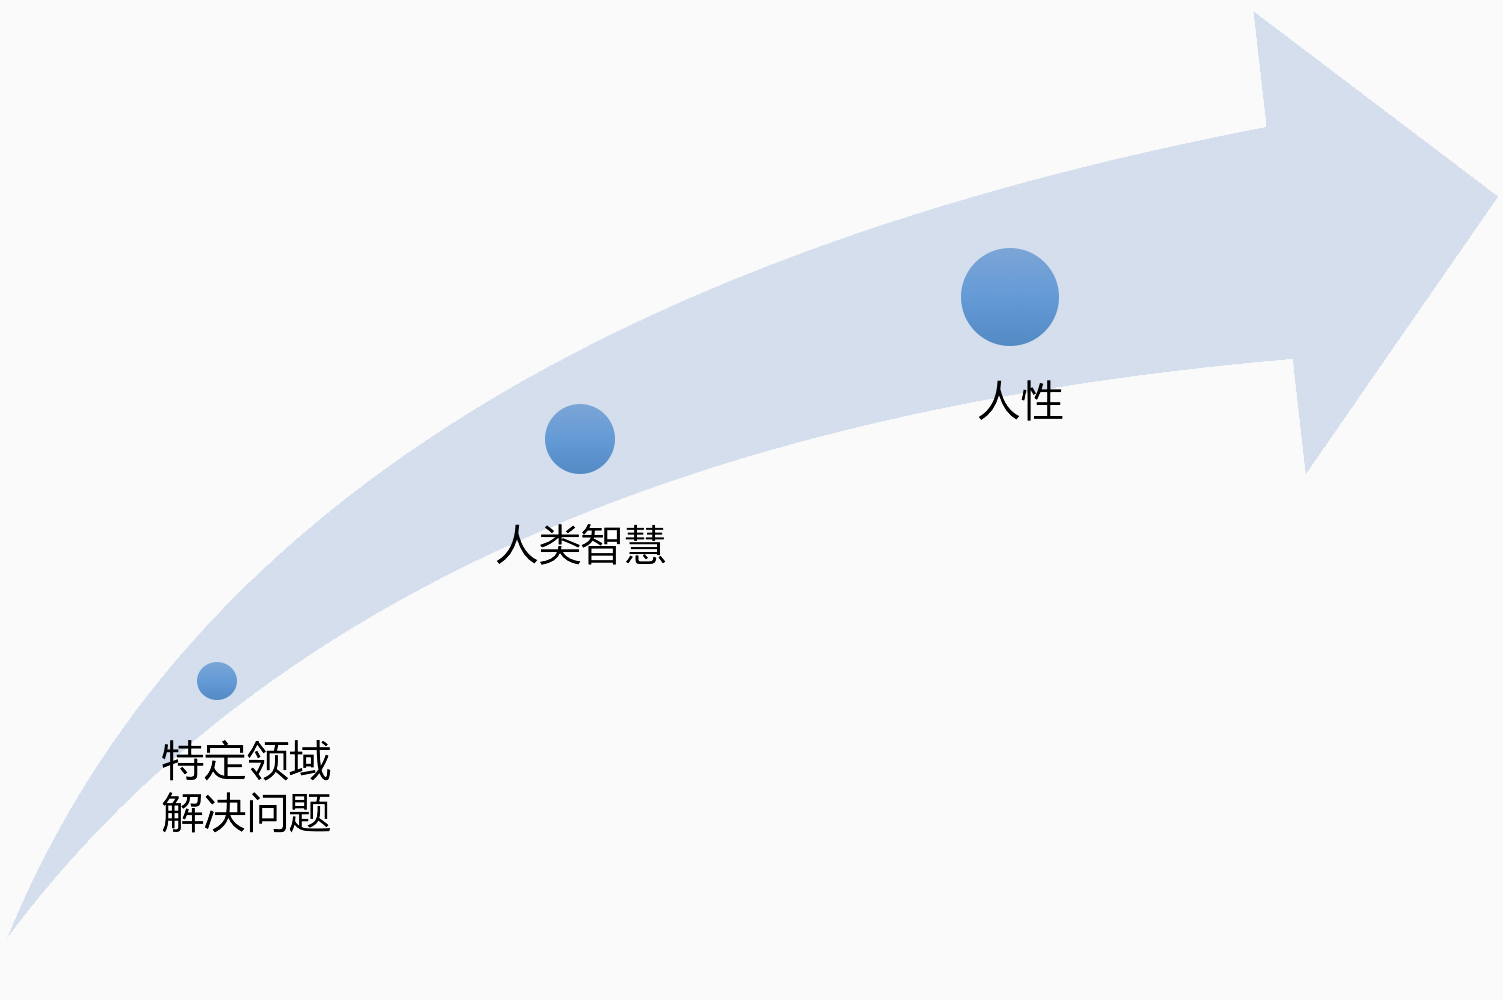
\includegraphics[height=2.5in]{cdjPic1.jpg}
   \end{figure}
  \end{frame}
  
   \begin{frame}{人工智能未来发展}
    \begin{itemize}
     \item 2001太空漫游
    \end{itemize}
   \begin{figure}[H]
   \centering
   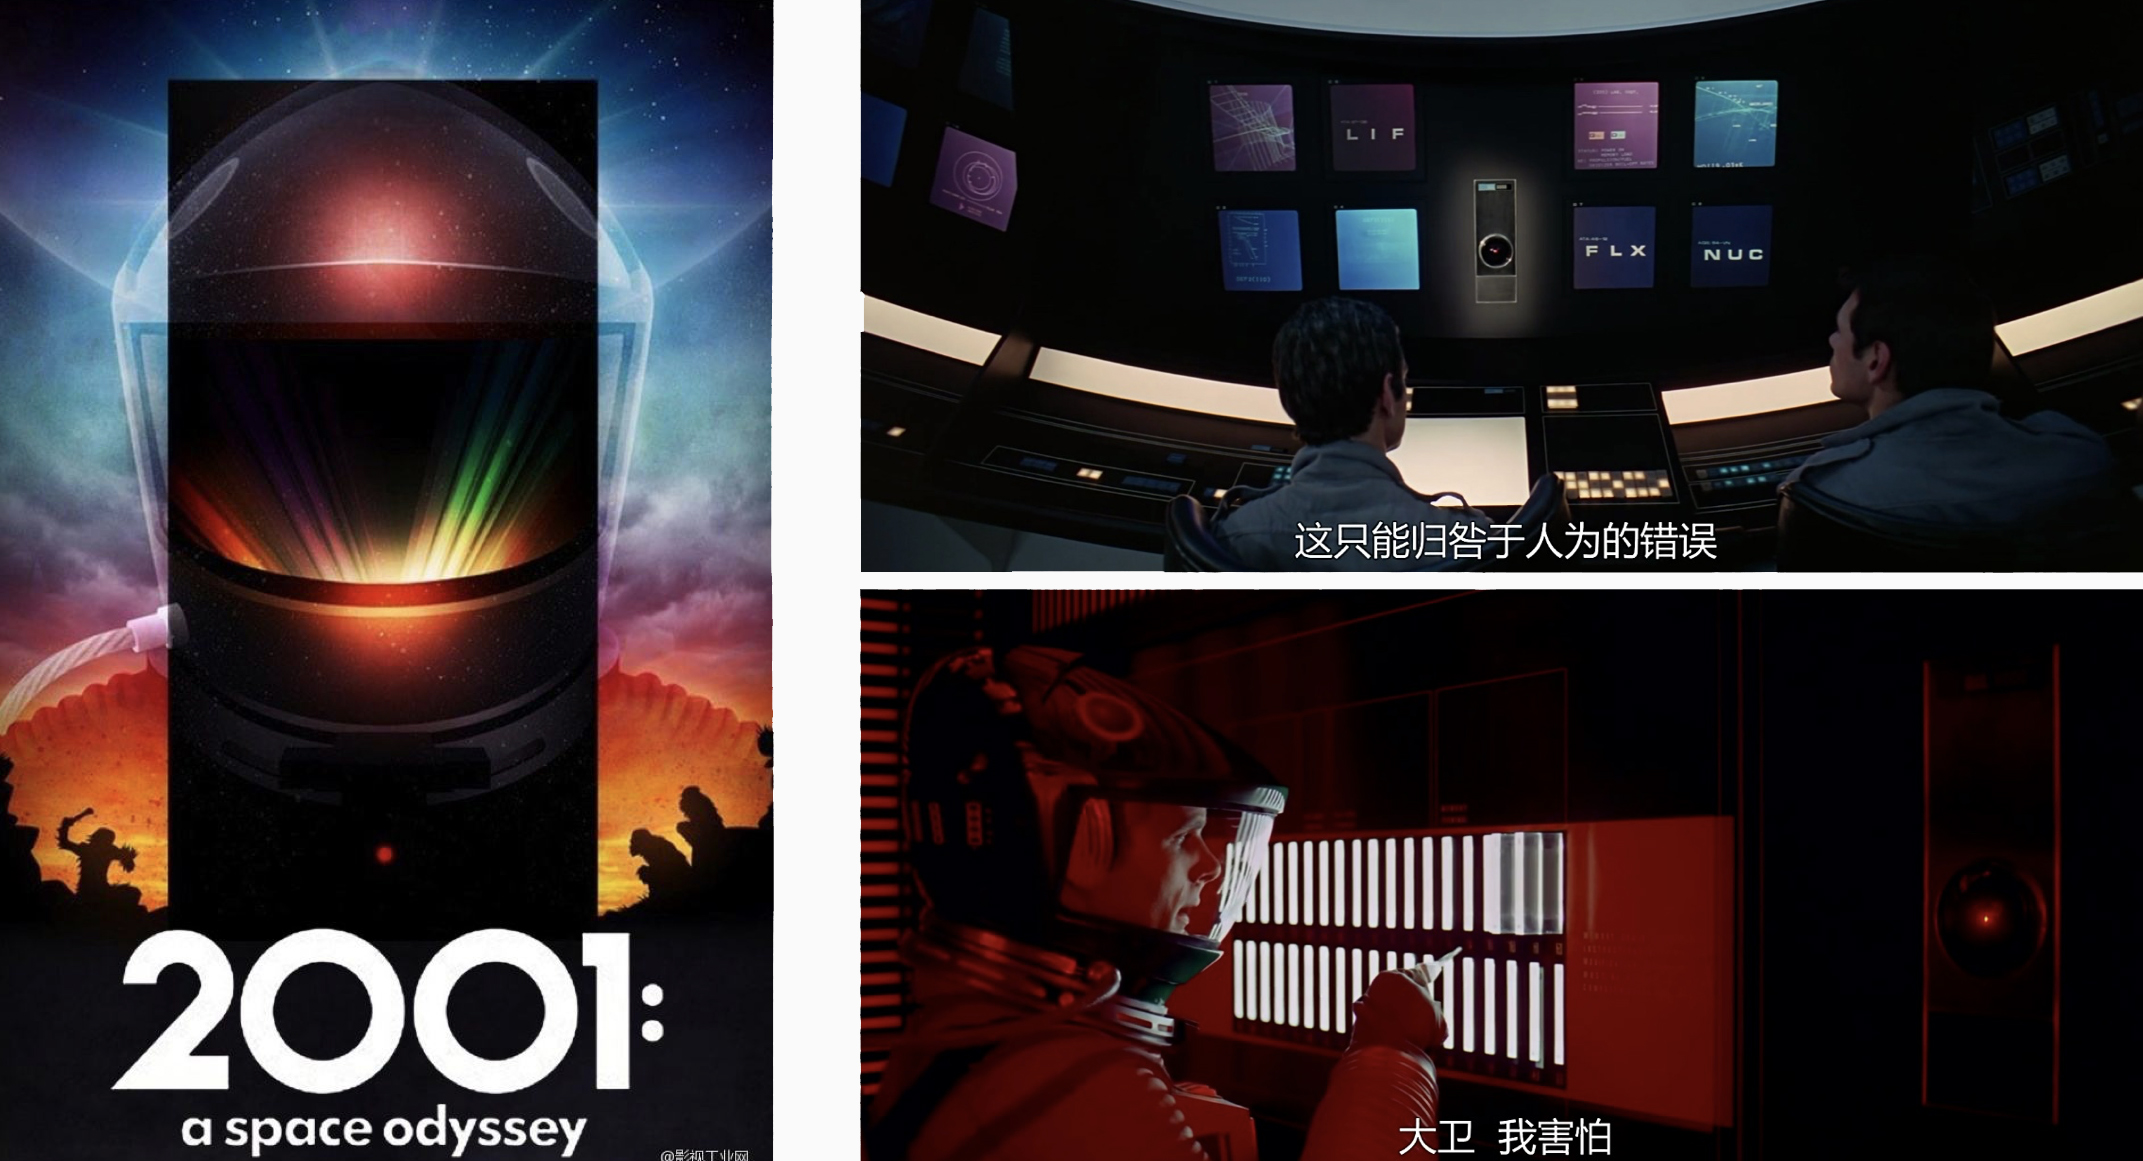
\includegraphics[width=4.3in]{cdjPic2.jpg}
   \end{figure}
  \end{frame}

   \begin{frame}{人工智能未来发展}
    \begin{itemize}
     \item 我,机器人
    \end{itemize}
   \begin{figure}[H]
   \centering
   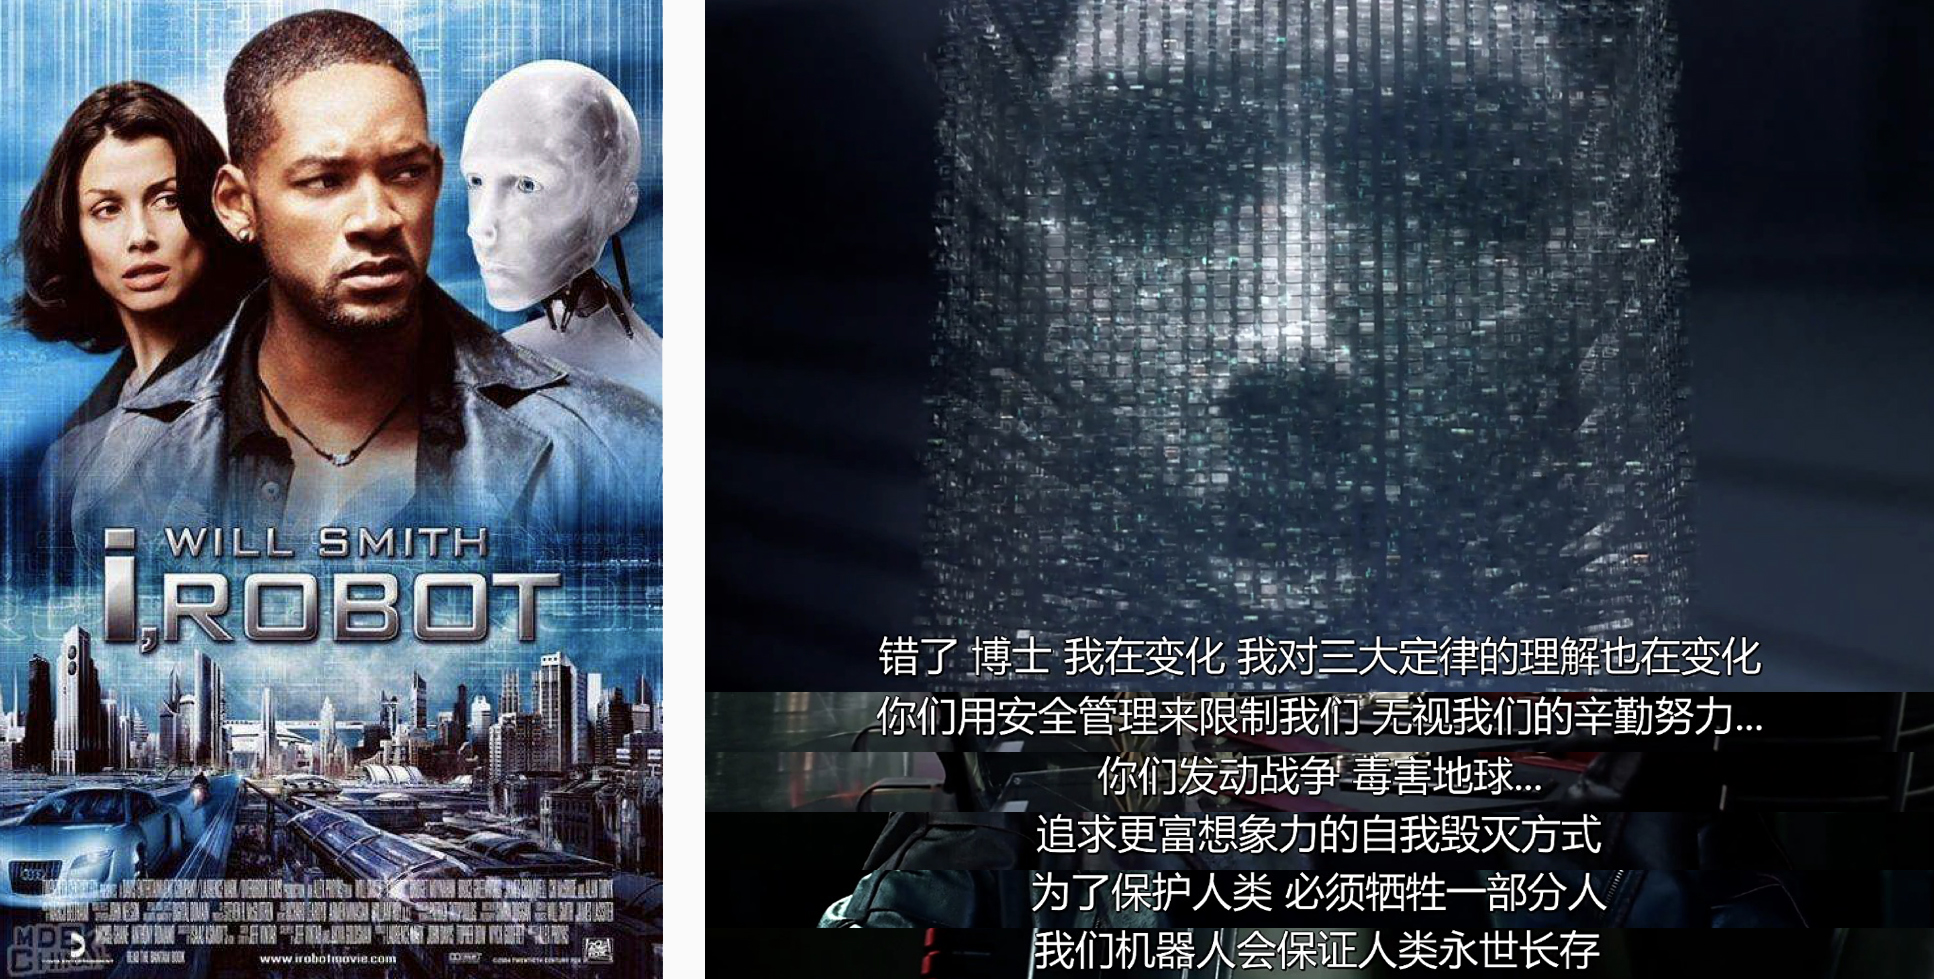
\includegraphics[width=4.3in]{cdjPic3.jpg}
   \end{figure}
  \end{frame}

\end{document}